\section{Possible methods}
\label{choiceOfMethod}

\subsection{Introduction}
In this section I will describe the different methods and algorithms I have used in this project, and discuss their merits and flaws.

Possible methods:

\begin{description}
\item[Computational Geometry:] The intuitive description of the Lonely Runner conjecture (\nref{introduction}) lends itself well to a geometrical interpretation, and leads me to wonder whether such an algorithm could efficiently find a solution.

\item[Number theoretic:] The Lonely Runner conjecture is, in its original formulation, a number theoretic problem. It is therefore reasonable to assume that a number theoretic approach would lead to an efficient verification program.
\end{description}

\subsection{Computational Geometry}
\label{compGeo}
The following solution is based on the first intuitive description of the conjecture, found in the introduction. It is clear that we are interested in the time interval when the runners are in the Zone, but not particularly where the individual runners are. We are only interested when a runner enters and leaves the Zone. 

Let $s$ be the speed of a given runner then the runner enters the Zone for the first time when he is $\frac{1}{n+1}$ units away from the start line, and leaves it when he has passed $\frac{n}{n+1}$ units.
Therefore the runner first enters the Zone at: 

\begin{equation}
\label{eqa:speedOne}
\begin{split}
s * t &= \frac{1}{n+1} \\
t &= \frac{1}{s * (n+1)}
\end{split}
\end{equation}

and leaves the Zone at time:

\begin{equation}
\label{eqa:speedTwo}
\begin{split}
s * t &= \frac{n}{n+1} \\
t &= \frac{n}{s * (n+1)}
\end{split}
\end{equation}

From \eqaref{eqa:speedOne} and \eqaref{eqa:speedTwo} it is clear that the time interval for the first time the runner is in the Zone will be 
\begin{displaymath}
\left[\frac{1}{s * (n+1)}, \frac{n}{s * (n+1)}\right]
\end{displaymath}

More generally, a runner with speed $s$ will be in the Zone for the $k$'th time, where $k \in \N \cup \E{0}$, in the time interval 

\begin{equation}
\label{eqa:genericZone}
\left[\frac{1 + k * (n+1)}{s * (n+1)}, \frac{n + k * (n+1)}{s * (n+1)}\right] 
\end{equation}

Now it becomes a matter find out whether there is a time where the time intervals for all the runners overlap. To do this I propose using a horizontal Plane Sweep algorithm\footnote{For a general overview of Plane Sweep algorithms, please consult \cite{citeulike:3347056} or any other university level or higher book dealing with Computational Geometry}, where the interesting cases are when a runner enters, and leaves the Zone. 

\subsubsection{High level description of the algorithm}

\begin{algorithm}[H]
  \caption{SimpleLonelyRunner}
  \highlights
  \SetKwData{and}{and}
  \Input{A list \s which contains n pairwise different speeds for n runners}
  \Output{A time \ti where all n runners are at least $\frac{1}{n + 1}$ units away from the starting line, or a \no, indicating that no such time exists}
  
  Make \finish with time $1$ and add it to \li

  \ForEach{speed $\in$ \s}{
    
    Make the first \startT and \eT based on speed - see \eqaref{eqa:speedOne} and \eqaref{eqa:speedTwo}, and insert it in \li
  }
  
  \While{\true}{

    Pop Event Point \p from \li
    
    \If{\p is \startT}{      
      
      Record that a runner has entered the Zone

      \If{all the runners are in the Zone}{
        \return $\p_{\ti}$
      }
    }
    
    \uElseIf{\p is \eT}{
      
      Record that a runner has left the Zone

      Make the next \startT and \eT based on \eT)
    }
    \ElseIf{\p is \finish}{
      \return \no
    }
  }
\end{algorithm}

See figure \ref{algoIlluImg} for an intuitive illustration of idea behind the algorithm. 

\begin{figure}[H]
  \centering
  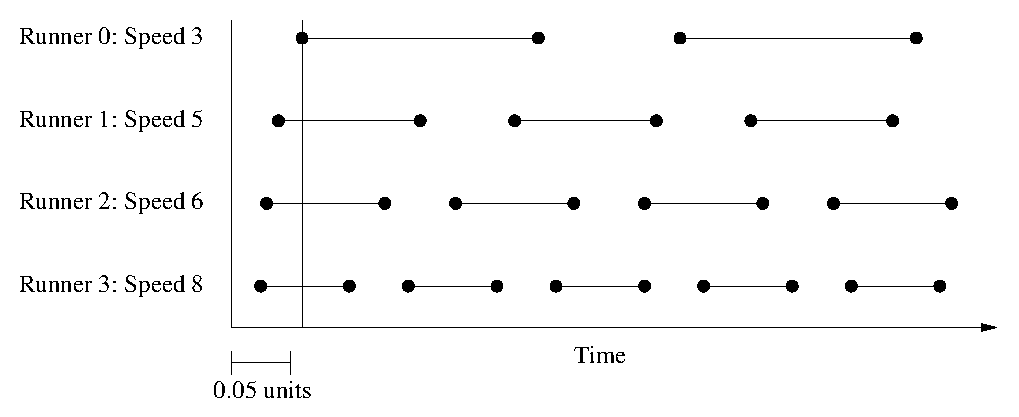
\includegraphics[width=\textwidth]{./images/algoIlluEPS}
  \caption{\label{algoIlluImg}An illustration of the Plane Sweep algorithm with the example speed of 3, 5, 6 and 9. The dots are the Event Points, and the horizontal line between Event Points are when a given runner is in the Zone. The Vertical line is the sweep line, which jumps from Event Point to Event Point from the left to the right, ignoring all time points in-between. The vertical line is here placed at the first time point that makes \eqaref{eqa:lonelyRunner} true for the speeds 3, 5, 6 and 9.}
\end{figure}

\subsubsection{Termination criteria}
\label{termination}
Since the Lonely Runner conjecture has not been proved for all $n \in \N$, there must be a means to terminate the algorithm, if for a given configuration of runners, there does not exists a time that make equation \eqaref{eqa:lonelyRunner} true.

My solution to this is to introduce the fake runner. The fake runner has a speed of $1$, and will only serve as a marker for when to terminate the algorithm. The intuition behind this is that based on equation \eqaref{eqa:lonelyRunner} - it is clear that if a solution exist it must do so for $x \in [0,1)$, and therefore if we reach the time $1$, no solution to equation \eqaref{eqa:lonelyRunner} exists.

\subsubsection{Event Points}
\label{eventPoints}
In this subsection I will discuss the role of Event Points in the Plane Sweep algorithm, as well as define them. 

As stated in Section \ref{compGeo} we are only interested in whether or not a runner is in the Zone, not his exact position on the track. To take advantage of this I introduce the Event Points, which are used to indicate whether a runner is entering, or leaving, the Zone, ignoring all other time points. 

One question that must be answered before we go any further, is whether or not we will create all Event Points before the main part of the algorithm begins\footnote{I have already established that we do not need to produce any Event Points that happen after time 1, it is clear that we can create all the Event Points before entering the main loop.} or create the first pair for each runner generate the remaining as it becomes necessary. This also has implications whether a Linked-List or a heap, respectively, should be used for the Priority Queue that will contain the Event Points. 

\adDis{
Creating all the Event Points in parallel before entering the main loop
}{
\item The advantage of creating the points in advance is that this can be done in parallel for each runner. After the point had been created, the main loop could be run without having to dedicate any resources to creating new events.

\item It would also make the Priority Queue simpler, since instead of a heap, we could simply use a Linked List structure. 
}{
\item Since all the points are generated at the beginning, this would sharply increase the memory footprint of the algorithm.

\item While the Event Points themselves could be generated in parallel, they would still have to be inserted into the Priority Queue, which would serve as a bottleneck. Even if this was done while the other Event Points were still being generated, it would slow down the procedure enormously, loosing a lot of time. The Priority Queue would still have to be sorted, which would take $O(k\log(k))$ time, where $k$ is the sum of all the runners speeds.

\item If done correctly it would add quite a bit of complexity to the program
}{
Given that generating an Event Point is a trivial operation (it being a very simple data structure), one can question the worth of this implementation.
}

\adDis{
Creating event points on the fly
}{
\item It would reduce the memory footprint drastically, as new event points would only be made when needed.

\item Adding the new event points sequentially would also be much simpler than in the parallel version, since there would be no need for locks to protect the Priority Queue needed.  
}{
\item Creating every Event Point sequentially could potentially take a lot more time than the parallel solution.
}{
Creating the event points on the fly is far simpler than making all the points before the algorithm starts, although it is potentially slower in situations where we have runners with large speeds, or where the solution to equation \eqaref{eqa:lonelyRunner} is close to $1$ or no solution to the equation exist for the given configuration of runners. 
}

Based on the above I would argue that creating the Event Points on the fly is the preferred solution, as any possible gains by creating all the Event Points in parallel before entering the main loop would be minimal at best\footnote{It is worth noting that the insertions and removals from the Priority Queue cannot be used as an argument either way, since the parallel and sequential version each uses a different data structure, optimised for their operation.}, and would unduly increase the complexity of the program. 

One important decision we have to make, is to decide how we are going to represent for the time of the various Event Points. From \eqaref{eqa:genericZone}, it is clear that the Event Points are going to have times that have real numbers. Based on the computer specifications I defined in Section \ref{specs} on page \pageref{specs}, it is clear that I do not want to have the algorithm rely on any special floating point number hardware, it would be nice if we could represent the time as an integer. 

Since the point of the time property of an Event Point is to compare it with the time of another Event Point, we must frame the comparison we are trying to make as follows: Let $n \in \N$ be the number of runners, $a_k \in \E{1, n}$ be the local position within in the Zone, let $k_k \in \N$ be the number of rounds runner $k$ has taken, and let $s_k \in \N$ be the speed of runner $k$, then if we are to compare Event Point i's to Event Point j's time, we have from \eqaref{eqa:genericZone}:
  
\begin{equation}
\label{eqa:integerTime}
\begin{split}
\frac{a_i + k_i * (n+1)}{s_i (n+1)} &< \frac{a_j + k_j * (n+1)}{s_j (n+1)} \Leftrightarrow\\
\frac{a_i + k_i * (n+1)}{s_i} &< \frac{a_j + k_j * (n+1)}{s_j} \Leftrightarrow\\
(a_i + k_i * (n+1)) * s_j &< (a_j + k_j * (n+1)) * s_i \Leftrightarrow
\end{split}
\end{equation}

So each Event Point must at least record its local position $a$, the number of rounds $k$ the runner has made, and the speed $s$ of the runner. Besides that, each Event Point should remember the number of its runner, so that all forms of ambiguity can be removed (see \ref{order}).

In order to distinguish entering and leaving the Zone, as well as the fake runner I introduce 3 different points:
\begin{description}
\item[\comStart] The first point represents the time where the runner is $\frac{1}{n + 1}$ units away from the start line.
\item[\comEnd] The first point after the \comStart\, where the runner is $\frac{1}{n + 1}$ units away from the start line. Since \comEnd\, is the last event point for any given runner in the Priority Queue, \comEnd\, will be used to signal that the algorithm must add new a \comStart\, and a \comEnd\ to the Priority Queue.
\item[\comFin] The final point in that will be processed --- which has set values of $a = n+1$, $k = 1$ and $s = 1$ and with its runner set to $n+1$. If this point is ever reached, then there exists no solution to \eqaref{eqa:lonelyRunner} for the given configuration of runners - and the configuration would serve as a counter example to the Lonely Runner conjecture.
\end{description}

\subsubsection{Order of points}
\label{order}
In order to avoid any ambiguity concerning the order of the points, I will now define an order $\prec$. \hide{One of the degenerate cases we need to avoid is when we have $(n-1)$ runners that are in the Zone, and the next two points are a \comEnd\, and a \comStart, both at the same time. Since the Zone is a closed set, it is clear that this instance should return a valid solution, but if \comEnd\, comes first, then the solution would not be reported - therefore \comStart\, must be placed before \comEnd.}

\begin{defi}[Order of points]
For the Event Points $p$ and $q$, $p \prec q$ iff
\begin{center}
\label{orderOfPoints}
$p_{time} < q_{time}$\\
or \\
$p_{time} = q_{time}$ and type($q$) = \comFin\\
or \\
$p_{time} = q_{time}$ and type($p$) = \comStart and type($q$) = \comEnd \\
or \\
$p_{time} = q_{time}$ and type($p$) = type($q$) and $p_{runner} < q_{runner}$
\end{center}
\end{defi}


\subsubsection{Algorithm}
\begin{algorithm}[H]
\caption{MakeTimePoints}
\highlights
\SetKwData{start}{startTime}
\Input{The old end point \p and the Event Point queue \li}
\Output{The time queue \li, with a new \startT and \eT inserted the runner \run}
 
Make new \startT $start$ from \p with all the same properties as \p, except that $start_{local position} = 1$ and $start_{rounds} = \p_{rounds} + 1$
  
Make new \eT $end$ from \p with all the same properties as \p, except that $end_{local position} = p_{number of runners}$ and $end_{rounds} = \p_{rounds} + 1$
    
Add $start$ and $end$ to \li

\return \li
\end{algorithm}

\begin{algorithm}[H]
  \caption{FindLonelyRunnerTime}
  \highlights
  \SetKwData{and}{and}
  \Input{A list \s which contains n pairwise different speeds for n runners}
  \Output{A point \p where all n runners are at least $\frac{1}{n + 1}$ units away from the starting line, or a \no, indicating that no such time exists}

  Create and initialise \li
  
  \inter $\gets 0$
  
  \n $\gets$ size(\s)
  
  $runnerNum \gets 1$
  
  Make the point \finish with the following properties: $\finish_{number of runners} = \n$, $\finish_{rounds} = 1$, $\finish_{speed} = 1$, $\finish_{\run} = \n + 1$, $\finish_{local position} = n + 1$, and add it to \li

  \ForEach{speed $\in$ \s}{
   
    Make the point \p with the following properties: $\finish_{number of runners} = \n$, $\finish_{rounds} = -1$, $\finish_{speed} = s$, $\finish_{\run} = runnerNum$, $\finish_{local position} = 0$

    \li $\gets$ MakeTimePoints(\p, \li)
    
    $runnerNum += 1$
  }
  
  \While{\li is not empty}{

    \p $\gets$ firstPoint(\li)
    
    \If{\p is \startT}{      
      \inter $+= 1$
    
      \If{\inter == \n}{
        \return $\p$
      }
    }
    
    \uElseIf{\p is \eT}{
    
      \inter $-= 1$
            
      \li $\gets$ MakeTimePoints(\p, \li)
    }
    \ElseIf{\p is \finish}{
      \return \no
    }
  }
\end{algorithm}

\subsubsection{Proofs of the Geometric algorithm}
\label{proof_geo}
\algProof{

The main idea of the algorithm is that it keeps track when runners enters and leaves the Zone, and iff it finds that all runners are in the Zone, then it reports the solution. The only way the algorithm can fail is therefore if either

\begin{description}
\item[Case A:] If a runner can enter the at time $t_{enter}$ Zone without the distance to the start line being $\frac{1}{n+1}$ units. 
\item[Case B:] If a runner can leave the at time $t_{leave}$ Zone without the shortest distance to the start line being $\frac{1}{n+1}$ units.  
\end{description}
Let $dist_r$(t): $\R \rightarrow [0, 1)$ be the distance function from the start line in the runners direction to the runner r at time t along the circular track.

Let entering the Zone at time $t_{enter}$ mean that $dist_r(t_{enter})$ is in the Zone, while $dist_r(t_{prev})$ is not in the Zone, where $t_{prev} = max\E{x \in \R: x < t_{enter}}$. Similarly let leaving the Zone at time $t_{leave}$ mean that $dist_r(t_{leave})$ is in the Zone, while $dist_r(t_{next})$ is not in the Zone, where $t_{next} = min\E{x \in \R: t_{leave} < x}$.
 
I will now prove that the runners always enters the Zone at $\frac{1}{n+1}$, and leaves it at $\frac{n}{n+1}$, so that case A and case B cannot happen, and thus my algorithm will always give the correct result.

I will now prove that case A cannot happen, by proof-by-contradiction:
Let us assume that the runner r enters the Zone at time $t_{enter}$, and that $dist_r(t_{enter}) \in (\frac{1}{n+1}, \frac{n}{n+1}]$. As defined above, there must therefore exist a time $t_{prev}$ just before $t_{enter}$ where $dist_r(t_{prev})$ is after the start line, but before the Zone. 

We now have a closed interval $[dist_r(t_{prev}), dist_r(t_{enter})]$, for which the function clearly is continues, it then follows from the Intermediate value theorem that there must exist a time $t_{real enter}$ where $dist_r(t_{real enter}) = \frac{1}{n+1}$. This however contradicts our assumption that the runner enters the Zone at $dist_r(t_{enter}) \in (\frac{1}{n+1}, \frac{n}{n+1}]$. Therefore it must follow that the runner always enters the Zone at distance $\frac{1}{n+1}$, which means that case A cannot happen, which was what I wanted to show.

Case B can be proved analogously, with $dist_r(t_{leave}) \in [\frac{1}{n+1}, \frac{n}{n+1})$, and $dist_r(t_{next})$ not being in the Zone.
}{
It is clear that the algorithm will always terminate, since the algorithm terminates when it finds \comFin\,(which cannot be removed prematurely).
}{
The first loop of the algorithm takes $O(n\log(n))$ time, since it has to add $2n$ event points to the Priority Queue, where each insertion taking $O(\log(n))$.\\

After the first loop, there will at most be $2n + 1$ or $O(n)$ Event Points in the Priority Queue, since each time we encounter a \comEnd, two new Event Points are added to the Priority Queue.\\ 

It is clear that the second loop is dependent on how many Event Points are processed before \comFin, at time $1$ is encountered. For any given runner with speed $s$, it is clear that it will make a $s$ rounds before the fake runner arrives at the finishing line, and each time  a runner makes a complete tour of the track, the algorithm has to deal with 2 Event Points --- a \comStart\; and an \comEnd. The \comStart\; event takes $O(1)$ to process, while the \comEnd will take $O(\log(n))$ time, because of Lemma 1\todo{introduce Lemma 1 - it should say that there will always be O(n) points in the heap}. Therefore it is clear that if we let  $k$ be the sum of all the runners speeds, then the algorithm has a time complexity of $O(k\log(n))$.
}

\subsection{Number Theory}
\label{numtheory:algo}
A Number Theory alternative to the Geometric Algorithm can be made by applying the results of \cite{invis}. I have sketched the algorithm described from \cite{invis} below. \cite{invis} studies the the function 
$$
k(D) = \sup_{x \in \R}\min_{1 \leq i \leq k}\Vert x d_i \Vert
$$
where D is a set $\E{d_1, d_2, \ldots, d_k}$ of integers. They arrive at the result that given D, $k(D)$ ``is attained for $x_0 = a /(d_i + d_j)$ for some $i \neq j$ and some positive integer a''. (Theorem 6 on page 66 in \cite{invis}). It is clear that $a < k$, since if $a = k$ then $a/k$ would evaluate to $1$ and then $\Vert \frac{a}{k} d\Vert, d \in D$ would evaluate to 0, and if $a > k$ then for $n \in \N: \Vert\frac{a}{k}\Vert = \Vert\frac{k+n}{k}\Vert = \Vert\frac{n}{k}\Vert$.

\begin{algorithm}[H]
  \caption{NumericalLonelyRunner}
  \highlights
  \SetKwData{and}{and}
  \Input{A list \s which contains n pairwise different speeds for n runners}
  \Output{A time \ti such that all n runners are at least $\frac{1}{n + 1}$ units away from the starting line, or a \no, indicating that no such time exists}
  
  $n \gets size(\s)$

  \For{$i \gets 1$ \KwTo $n-1$}{
    
    $d \gets \s_i$
 
    \For{$j \gets i + 1$ \KwTo $n$}{
      
      $d^{\prime} \gets \s_j$

      $k \gets d + d^{\prime}$
      
      \For{$a \leftarrow 1$ \KwTo $k-1$}{
        
        $testValid \gets true$
        
        \ForEach{$s \in \s$}{
          
          $testValid \gets testValid\; \and\; (\Vert \frac{a}{k} * s \Vert \geq \frac{1}{n+1} )$

          \If{!$testValid$} {
            break
            }
          
        }
        
        \If{testValid}{
          
          \return $\frac{a}{k}$
          
        }
      }
    }
  }
  \return \no
\end{algorithm}

Since the algorithm in worst case tries every single combination of
$d$ and $d\prime$, and \cite{invis} describes no way to detect which
values of $d$ and $d\prime$ that may be candidates for a possible
solution. It is therefore clear that the run-time of the Numerical
algorithm must be dependent on the order of the runner speeds in speeds.

\subsubsection{Proofs for the numerical algorithm}
\label{proof_num}
\algProof{
This algorithm builds on Theorem 6 in \cite{invis}. Theorem 6 says that if we have a finite set of positive integers D = $\E{d_1, d_2, \ldots, d_k}$, then  $\kappa(D) = \sup_{x \in \R}\min_{1\leq i \leq k}\Vert x d_i \Vert$ is achieved for $x_o = a/(d_i + d_j)$ for some $0 \leq i,j \leq k, i \neq j$, and some positive integer a. I will now paraphrase the proof for this from \cite{invis}:

Let us look at the function $f_D(x) = \min_{1 \leq i \leq k}\Vert x d_i \Vert$. Let $x_0$ be the value that maximises $f_D$, where $x_0 \in \mathbb{T}$, where $\mathbb{T} = [0;1)$, which is the circle. Such an $x_0$ must exist since $f_D$ is continues, and the circle (and hence) $\mathbb{T}$ is compact. Thus we have $\kappa(D) = f_D(x_0) = \min_{1 \leq i \leq k} \Vert x_0 d_i \Vert$. Let $d_j \in D$ be a value that minimises $\kappa(D)$ and $f_D(x_0)$. We now have that $\kappa(D) = \Vert x_0 d_j\Vert$. 
Furthermore, since all the functions we are dealing with are continues, there must exist a $d_i \in D$, where $j \neq i$, such that $\Vert x_0 d_j \Vert = \Vert x_0 d_i \Vert$. I will prove that this is the case by proof by contradiction:

Let us assume that $x_0$ such that $\kappa(D) = \Vert x_0 d_j \Vert$, for some $d_j \in D$, and that no $d_i$ exist such that $\Vert x_0 d_j \Vert = \Vert x_0 di\Vert$. In that case, we must have that for all $d_m \in D, m \neq j: \Vert x_0 d_m \Vert > \Vert x_0 d_j$, since we explicitly found $d_j$ to be the value that minimizes $f_D(x_0)$. Then, since $f_D$ is continues, we can take $y = x_0 \pm \epsilon$ for a small value $\epsilon > 0$, and since $d_j$ was the only value that minimised $f_D(x_0)$, and changing the value of $x_0$ by $\epsilon$ will not change that, we can increase value of $f_D$ so that $f_D(y) > f_D(x_0)$. However, this contradicts our initial assumption that $x_0$ maximises $f_D$, and therefore there must exist a $d_i$ such that $\Vert x_0 d_i \Vert = \Vert x_0 d_j \Vert$.  
 
In fact we have the case $\E{x_0 d_j} = 1 - \E{x_0 d_i}$, where $\E{x}$ is the fractional part of x, i.e. the position on the circle. Thus we have 

\begin{equation}
\begin{split}
x_0d_j + x_0d_i &= \lfloor x_0d_j \rfloor + \E{x_0d_j} + \lfloor x_0d_i \rfloor + \E{x_0d_i} \\
               &= \lfloor x_0d_j \rfloor + \lfloor x_0d_i \rfloor + 1 = a
\end{split} 
\end{equation}

which we can rearrange into $x_0 = a / (d_j + d_i)$, which indeed gives us $\kappa(D)$, which was what we wanted to show.

\cite{invis} then uses this to prove that their Conjecture 5 is equivalent to the Lonely Runner conjecture, and shows how the finding the value of a will solve their conjecture if the Lonely Runner conjecture holds.

In order to make sure that the Numerical algorithm will always terminate, even in the case where the Lonely Runner conjecture does not hold, I have added the last return statement, ensuring that the correct answer will always be reported.
}{
It is clear that the algorithm will always terminate, $\Vert x \Vert $ is the only function call in the algorithm, and it will always terminate.
}{
It is clear that the meat of NumericalLonelyRunner is 4 nested for-loops. The 2 first loops are dependent on each other, the third is based on the speed for the two runners that have been chosen, and the last loop goes through all the runners.\\

The first 2 loops gives us $\sum_{i=1}^{n-1}\sum_{j=i+1}^{n}1 = n-1 + n-2 + \ldots 2 + 1$, which reduces to $O(n^2)$. The third loop must iterate $k-1$ times, where $k$ is the sum of 2 runner's speed.\\

If we are to give a worst case time, then it is clear $k$ must be the sum of the speed of the two fastest runners - so if we let $speed_1 = max(\comS)$ and $speed_2 = max(\comS \setminus \E{speed_1})$ then $k = speed_1 + speed_2$
And we go through the last loop $n$ times. Thus the entire algorithm runs in $O(k * n^3)$.
}

\subsection{Conclusion}

From the above we results we can see that neither of the algorithm are better in all cases. The Geometrical algorithm has a better worst case time complexity when we have many runners with low speeds, while the numerical algorithm is better when we have few runners with very high speeds. It is also clear that the numerical algorithm is far easier to implement, relying on no non-standard data structures.

However, since they both are very short, and do not have much in the way of dependencies, I will try to implement them both and compare their run-times for a variety number of runners and speeds. 

In this section I have presented 2 different methods that can be used to decide whether equation \eqaref{eqa:lonelyRunner} is true for a given configuration. I have analysed their run-times and given proofs that they will always terminate, and that they will return the correct solution to equation \eqaref{eqa:lonelyRunner}, if one such exists, and otherwise inform the caller that no such value exists.
